\chapter{CONTEXTE GÉNÉRAL DU PROJET}
\label{ch:contexte}

Ce chapitre présente le cadre professionnel du Projet de Fin d'Études, l'organisme d'accueil, le contexte client et la démarche de conduite adoptée. Il permet de situer la contribution technique dans un environnement réel de transformation digitale et de data engineering.

%==============================================================================
\section{Organisme d'accueil : SEVENAPP}
%==============================================================================

\textbf{SEVENAPP}, opérant sous la marque \textbf{Seven}, est une entreprise de services numériques spécialisée dans l'accompagnement des organisations autour de la transformation digitale, de la data et de l'intelligence artificielle. Son positionnement consiste à intervenir comme partenaire technologique auprès d'acteurs publics et privés, en mettant à disposition des consultants capables de concevoir, industrialiser et documenter des solutions numériques.

\begin{figure}[H]
\centering
\maybeimage[height=2cm]{images/seven-logo.jpg}
\caption{Logo SEVENAPP}
\label{fig:seven-logo}
\end{figure}

Dans le cadre de ce stage, le rôle occupé est celui de \textbf{consultant Data}. La mission s'inscrit dans une logique d'ingénierie : comprendre un besoin de plateforme, proposer une architecture, produire une implémentation reproductible, documenter les choix et préparer une démonstration technique.

\subsection{Fiche signalétique}

\begin{table}[H]
\centering
\caption{Fiche signalétique de SEVENAPP}
\label{tab:fiche-sevenapp}
\PFETableSetup
\rowcolors{2}{tablealt}{white}
\begin{tabularx}{\textwidth}{@{}p{0.28\textwidth}Y@{}}
\rowcolor{tableheader}
\PFEHeaderCell{Élément} & \PFEHeaderCell{Description} \\
\midrule
\PFEKeyCell{Dénomination} & SEVENAPP, opérant sous la marque Seven \\
\PFEKeyCell{Nature} & Entreprise de Services du Numérique orientée Digital, Data et Intelligence Artificielle \\
\PFEKeyCell{Date de création} & 2018 \\
\PFEKeyCell{Siège} & Casablanca, Maroc \\
\PFEKeyCell{Positionnement} & Accompagnement des organisations dans la transformation digitale, l'industrialisation des produits data et l'intégration de solutions innovantes \\
\PFEKeyCell{Domaines d'expertise} & Consulting, Digital, Data, Intelligence Artificielle, plateformes banking, Data Lakehouse et IA générative \\
\PFEKeyCell{Effectif public communiqué} & Plus de 45 consultants et experts \\
\PFEKeyCell{Rôle dans le projet} & Organisme d'accueil du stage et cadre de réalisation de la mission de consultant Data auprès d'EQDOM \\
\bottomrule
\end{tabularx}
\end{table}

\subsection{Domaines d'intervention}

Les activités de l'organisme d'accueil peuvent être regroupées autour de trois axes :
\begin{itemize}
    \item \textbf{transformation digitale} : modernisation des processus, intégration d'applications et accompagnement métier ;
    \item \textbf{data engineering} : pipelines, plateformes, gouvernance, ingestion, transformation et exposition des données ;
    \item \textbf{intelligence artificielle} : exploitation avancée des données, automatisation et cas d'usage analytiques.
\end{itemize}

\begin{figure}[H]
\centering
\maybeimage[width=0.82\textwidth]{images/sect_act_seven.png}
\caption{Domaines d'intervention de SEVENAPP}
\label{fig:secteurs-activite-seven}
\end{figure}

\subsection{Références clients}

La diversité des références clients de SEVENAPP illustre son positionnement transversal auprès d'acteurs financiers, d'organismes publics et d'entreprises issues de secteurs variés. Ces missions couvrent notamment la refonte de parcours digitaux, la mise en place de solutions CRM, la structuration de dispositifs data, l'automatisation de processus et l'accompagnement à la gouvernance des données.

\begin{figure}[H]
\centering
\maybeimage[height=0.72\textheight,keepaspectratio]{images/Clients.png}
\caption{Exemples de références clients de SEVENAPP}
\label{fig:clients-sevenapp}
\end{figure}

\subsection{Organigramme simplifié}

\begin{figure}[H]
\centering
\resizebox{0.95\textwidth}{!}{%
\begin{tikzpicture}[
    box/.style={rectangle, rounded corners=2pt, draw=tocblueblack, fill=lightpanel, align=center, minimum height=0.9cm, text width=3.2cm, font=\small},
    main/.style={box, fill=white, line width=0.8pt, text width=4.2cm, font=\small\bfseries},
    arr/.style={-{Latex[length=2mm]}, draw=tocblueblack}
]
\node[main] (dir) {Direction générale};
\node[box, below left=1.1cm and 2.6cm of dir] (consulting) {Pôle Consulting\\Stratégie et cadrage};
\node[box, below=1.1cm of dir] (digital) {Pôle Digital\\Applications et produits};
\node[box, below right=1.1cm and 2.6cm of dir] (data) {Pôle Data \& IA\\Plateformes, BI et IA};
\node[box, below=1.1cm of digital] (support) {Fonctions support\\RH, administratif, commercial};
\draw[arr] (dir) -- (consulting);
\draw[arr] (dir) -- (digital);
\draw[arr] (dir) -- (data);
\draw[arr] (dir) -- (support);
\end{tikzpicture}
}
\caption{Organigramme simplifié de SEVENAPP}
\label{fig:organigramme-sevenapp}
\end{figure}

%==============================================================================
\section{Contexte client : EQDOM}
%==============================================================================

\subsection{Présentation du client}

\textbf{EQDOM} est un acteur marocain du financement et du crédit à la consommation. Son activité repose sur la gestion de parcours clients, de dossiers de financement, de données opérationnelles et d'indicateurs de pilotage. Dans ce type d'environnement, la donnée joue un rôle central : elle alimente l'analyse du risque, le suivi commercial, la conformité, le reporting interne et les tableaux de bord décisionnels.

\begin{figure}[H]
\centering
\maybeimage[height=2cm]{images/eqdom-logo.png}
\caption{Logo EQDOM}
\end{figure}

\subsection{Fiche signalétique}

\begin{table}[H]
\centering
\caption{Fiche signalétique d'EQDOM}
\label{tab:fiche-eqdom}
\PFETableSetup
\rowcolors{2}{tablealt}{white}
\begin{tabularx}{\textwidth}{@{}p{0.30\textwidth}Y@{}}
\rowcolor{tableheader}
\PFEHeaderCell{Élément} & \PFEHeaderCell{Description} \\
\midrule
\PFEKeyCell{Dénomination sociale} & EQDOM \\
\PFEKeyCell{Forme juridique} & Société anonyme à Conseil d'Administration \\
\PFEKeyCell{Date de création} & Septembre 1974 \\
\PFEKeyCell{Siège social} & 127, Boulevard Zerktouni, Casablanca \\
\PFEKeyCell{Secteur d'activité} & Crédit à la consommation et financement automobile \\
\PFEKeyCell{Produits principaux} & Prêts personnels, crédit automobile, financement d'équipement et solutions de crédit affecté \\
\PFEKeyCell{Réseau commercial} & 24 agences réparties dans les principales villes du Royaume, complétées par des intermédiaires agréés et des partenaires distributeurs \\
\PFEKeyCell{Contexte de la mission} & Client final de la mission Data portée par SEVENAPP, avec un besoin de modernisation et de fiabilisation des flux de données \\
\bottomrule
\end{tabularx}
\end{table}

\subsection{Aperçu historique}

EQDOM est considérée comme l'une des premières sociétés marocaines spécialisées dans le financement et le crédit à la consommation. Créée en 1974 à l'initiative de la Société Nationale d'Investissement et de la Caisse de Dépôt et de Gestion, elle avait initialement pour vocation de faciliter l'acquisition de biens d'équipement par les ménages marocains et de soutenir le développement du secteur de l'électroménager.

L'entreprise a connu une première étape structurante en 1978 avec son introduction à la Bourse de Casablanca. À partir des années 1990, EQDOM a engagé une dynamique d'élargissement de son activité, marquée par la diversification de ses produits et l'extension progressive de son réseau d'agences. Cette évolution lui a permis de passer d'un positionnement centré sur le financement d'équipement à une offre plus large couvrant les prêts personnels, le crédit automobile et les solutions de financement affecté.

Dans les années 2000, l'entreprise a renforcé son ancrage dans le secteur financier marocain à travers son adossement à un groupe bancaire de référence. Plus récemment, l'évolution du paysage bancaire marocain et les opérations de réorganisation actionnariale ont inscrit EQDOM dans une nouvelle phase de transformation. Dans ce contexte, la donnée devient un levier essentiel pour améliorer le pilotage commercial, fiabiliser le reporting, suivre les risques et accompagner la digitalisation des parcours clients.

\subsection{Organigramme simplifié}

\begin{figure}[H]
\centering
\definecolor{orgprimary}{RGB}{23,72,86}
\definecolor{orgsecondary}{RGB}{34,122,118}
\definecolor{orgaccent}{RGB}{218,96,76}
\definecolor{orgsoft}{RGB}{247,250,249}
\definecolor{orgline}{RGB}{35,67,79}
\resizebox{0.98\textwidth}{!}{%
\begin{tikzpicture}[
    orgdark/.style={rectangle, rounded corners=4pt, draw=orgprimary, fill=orgprimary, text=white, align=center, minimum height=0.78cm, text width=4.05cm, inner xsep=5pt, inner ysep=4pt, font=\sffamily\footnotesize\bfseries},
    orgbox/.style={rectangle, rounded corners=4pt, draw=orgline, fill=orgsoft, text=orgline, align=center, minimum height=0.78cm, text width=3.05cm, inner xsep=5pt, inner ysep=4pt, font=\sffamily\footnotesize},
    orgaccentbox/.style={rectangle, rounded corners=4pt, draw=orgsecondary, fill=orgsecondary, text=white, align=center, minimum height=0.78cm, text width=4.05cm, inner xsep=5pt, inner ysep=4pt, font=\sffamily\footnotesize\bfseries},
    orgfocus/.style={orgbox, draw=orgaccent, fill=orgaccent!6, line width=1pt, text width=3.05cm, font=\sffamily\footnotesize\bfseries},
    link/.style={draw=orgline, line width=0.5pt}
]
\node[orgdark] (ca) at (0,0) {Conseil d'Administration};
\node[orgdark, below=0.78cm of ca] (dg) {Direction générale};

\node[orgbox] (commerce) at (-6.0,-3.1) {Direction commerciale\\Réseau et partenariats};
\node[orgbox] (risque) at (-2.0,-3.1) {Direction risques\\Conformité et contrôle};
\node[orgdark] (ops) at (2.0,-3.1) {Direction opérations\\Crédits et back-office};
\node[orgbox] (finance) at (6.0,-3.1) {Direction financière\\Pilotage et reporting};

\node[orgaccentbox, below=1.25cm of ops] (sidata) {Direction SI / Data};

\node[orgbox] (apps) at (-5.1,-6.65) {Applications\\métiers};
\node[orgbox] (data) at (-1.7,-6.65) {Data\\et reporting};
\node[orgbox] (infra) at (1.7,-6.65) {Infrastructure\\et sécurité};
\node[orgfocus] (lakehouse) at (5.1,-6.65) {Plateforme\\Lakehouse};

\begin{pgfonlayer}{background}
\draw[link] (ca.south) -- (dg.north);
\draw[link] (-6.0,-2.25) -- (6.0,-2.25);
\draw[link] (-6.0,-2.25) -- (commerce.north);
\draw[link] (-2.0,-2.25) -- (risque.north);
\draw[link] (2.0,-2.25) -- (ops.north);
\draw[link] (6.0,-2.25) -- (finance.north);
\draw[link] (ops.south) -- (sidata.north);
\draw[link] (sidata.south) -- (2.0,-6.02);
\draw[link] (-5.1,-6.02) -- (5.1,-6.02);
\draw[link] (-5.1,-6.02) -- (apps.north);
\draw[link] (-1.7,-6.02) -- (data.north);
\draw[link] (1.7,-6.02) -- (infra.north);
\draw[link] (5.1,-6.02) -- (lakehouse.north);
\end{pgfonlayer}
\draw[link] (dg.south) -- (0,-2.25);
\end{tikzpicture}
}
\caption{Organigramme simplifié d'EQDOM}
\label{fig:organigramme-eqdom}
\end{figure}

\subsection{Réseau d'agences}

EQDOM s'appuie sur un réseau de distribution directe afin d'assurer une présence de proximité auprès de ses clients, de ses partenaires automobiles et des organismes conventionnés. La documentation institutionnelle consultée indique un total de \textbf{24 agences} réparties dans les principales villes du Royaume.

\begin{table}[H]
\centering
\caption{Répartition des agences EQDOM par ville}
\label{tab:agences-eqdom}
\PFETableSetup
\rowcolors{2}{tablealt}{white}
\begin{tabularx}{0.86\textwidth}{@{}XrXr@{}}
\rowcolor{tableheader}
\PFEHeaderCell{Ville} & \PFEHeaderCell{Agences} & \PFEHeaderCell{Ville} & \PFEHeaderCell{Agences} \\
\midrule
\PFEKeyCell{Casablanca} & 6 & \PFEKeyCell{Rabat} & 3 \\
\PFEKeyCell{Marrakech} & 2 & \PFEKeyCell{Tanger} & 2 \\
\PFEKeyCell{Settat} & 1 & \PFEKeyCell{Fès} & 1 \\
\PFEKeyCell{Salé} & 1 & \PFEKeyCell{Oujda} & 1 \\
\PFEKeyCell{Agadir} & 1 & \PFEKeyCell{Safi} & 1 \\
\PFEKeyCell{Tétouan} & 1 & \PFEKeyCell{Meknès} & 1 \\
\PFEKeyCell{El Jadida} & 1 & \PFEKeyCell{Kénitra} & 1 \\
\PFEKeyCell{Béni Mellal} & 1 & \PFEKeyCell{Total} & \textbf{24} \\
\bottomrule
\end{tabularx}
\end{table}

\begin{figure}[H]
\centering
\resizebox{0.88\textwidth}{!}{%
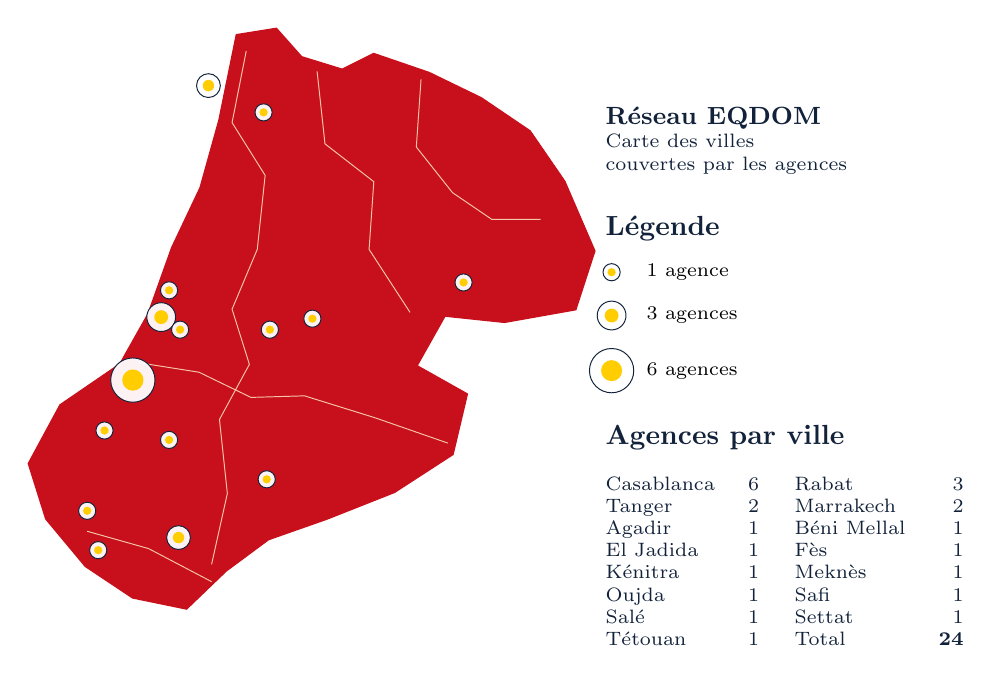
\begin{tikzpicture}[every node/.style={font=\scriptsize}]
    \definecolor{mapfill}{RGB}{200,16,28}
    \definecolor{mapline}{RGB}{18,34,58}
    \definecolor{mapborder}{RGB}{255,229,194}
    \definecolor{mapdot}{RGB}{255,205,0}
    \definecolor{mapmuted}{RGB}{92,96,106}

    % Silhouette schématique centrée sur la zone où EQDOM dispose d'agences.
    \filldraw[fill=mapfill, draw=mapfill, line width=0.9pt]
        (4.34,14.56) -- (4.84,14.64) -- (5.16,14.28) -- (5.68,14.12)
        -- (6.08,14.32) -- (6.78,14.08) -- (7.44,13.76) -- (8.06,13.34)
        -- (8.50,12.70) -- (8.88,11.82) -- (8.64,11.08) -- (7.74,10.92)
        -- (6.98,11.00) -- (6.62,10.36) -- (7.26,10.00) -- (7.08,9.24)
        -- (6.34,8.76) -- (5.48,8.42) -- (4.74,8.16) -- (4.20,7.76)
        -- (3.70,7.28) -- (3.02,7.42) -- (2.42,7.82) -- (1.92,8.42)
        -- (1.70,9.12) -- (2.10,9.86) -- (2.86,10.38) -- (3.22,11.02)
        -- (3.52,11.86) -- (3.88,12.62) -- (4.12,13.48) -- cycle;

    % Limites administratives stylisées pour rappeler la carte de référence.
    \draw[mapborder, line width=0.35pt, opacity=0.85]
        (4.46,14.36) -- (4.28,13.45) -- (4.70,12.78) -- (4.60,11.84)
        -- (4.28,11.08) -- (4.50,10.38) -- (4.12,9.68) -- (4.22,8.74)
        -- (4.02,7.84);
    \draw[mapborder, line width=0.35pt, opacity=0.85]
        (5.36,14.10) -- (5.46,13.18) -- (6.08,12.70) -- (6.02,11.84)
        -- (6.54,11.04);
    \draw[mapborder, line width=0.35pt, opacity=0.85]
        (6.68,14.00) -- (6.62,13.14) -- (7.08,12.56) -- (7.58,12.22)
        -- (8.20,12.22);
    \draw[mapborder, line width=0.35pt, opacity=0.85]
        (3.10,10.40) -- (3.86,10.28) -- (4.52,9.96) -- (5.20,9.98)
        -- (6.10,9.70) -- (7.02,9.38);
    \draw[mapborder, line width=0.35pt, opacity=0.85]
        (2.44,8.26) -- (3.22,8.04) -- (4.02,7.62);
    \node[anchor=west, font=\small\bfseries, text=mapline] at (8.90,13.50) {Réseau EQDOM};
    \node[anchor=west, align=left, text=mapline] at (8.90,13.05) {Carte des villes\\couvertes par les agences};

    \newcommand{\agencycity}[3]{%
        \fill[white, opacity=0.95] (#1,#2) circle[radius=#3];
        \fill[mapdot] (#1,#2) circle[radius=0.48*#3];
        \draw[mapline, line width=0.35pt] (#1,#2) circle[radius=#3];
    }

    % Points proportionnels au nombre d'agences.
    \agencycity{3.98}{13.92}{4.3pt}
    \agencycity{4.68}{13.58}{3.1pt}
    \agencycity{3.48}{11.32}{3.1pt}
    \agencycity{3.38}{10.98}{5.2pt}
    \agencycity{3.62}{10.82}{3.1pt}
    \agencycity{3.02}{10.18}{8.0pt}
    \agencycity{2.66}{9.54}{3.1pt}
    \agencycity{2.44}{8.52}{3.1pt}
    \agencycity{3.48}{9.42}{3.1pt}
    \agencycity{4.76}{10.82}{3.1pt}
    \agencycity{5.30}{10.96}{3.1pt}
    \agencycity{7.22}{11.42}{3.1pt}
    \agencycity{4.72}{8.92}{3.1pt}
    \agencycity{3.60}{8.18}{4.3pt}
    \agencycity{2.58}{8.02}{3.1pt}

    % Légende.
    \node[anchor=west, font=\bfseries, text=mapline] at (8.90,12.10) {Légende};
    \fill[white, opacity=0.95] (9.10,11.55) circle[radius=3.1pt];
    \fill[mapdot] (9.10,11.55) circle[radius=1.5pt];
    \draw[mapline, line width=0.35pt] (9.10,11.55) circle[radius=3.1pt];
    \node[anchor=west] at (9.42,11.55) {1 agence};
    \fill[white, opacity=0.95] (9.10,11.00) circle[radius=5.2pt];
    \fill[mapdot] (9.10,11.00) circle[radius=2.5pt];
    \draw[mapline, line width=0.35pt] (9.10,11.00) circle[radius=5.2pt];
    \node[anchor=west] at (9.42,11.00) {3 agences};
    \fill[white, opacity=0.95] (9.10,10.30) circle[radius=8.0pt];
    \fill[mapdot] (9.10,10.30) circle[radius=3.8pt];
    \draw[mapline, line width=0.35pt] (9.10,10.30) circle[radius=8.0pt];
    \node[anchor=west] at (9.42,10.30) {6 agences};
    \node[anchor=west, font=\bfseries, text=mapline] at (8.90,9.45) {Agences par ville};
    \node[anchor=north west, text=mapline] at (8.90,9.10) {%
        \begin{tabular}{@{}lr@{\hspace{0.45cm}}lr@{}}
        Casablanca & 6 & Rabat & 3 \\
        Tanger & 2 & Marrakech & 2 \\
        Agadir & 1 & Béni Mellal & 1 \\
        El Jadida & 1 & Fès & 1 \\
        Kénitra & 1 & Meknès & 1 \\
        Oujda & 1 & Safi & 1 \\
        Salé & 1 & Settat & 1 \\
        Tétouan & 1 & Total & \textbf{24}
        \end{tabular}
    };
\end{tikzpicture}
}
\caption{Carte schématique des villes couvertes par les agences EQDOM}
\label{fig:carte-agences-eqdom}
\end{figure}

\subsection{Enjeux data du contexte financier}

Le contexte financier impose des exigences particulières :
\begin{itemize}
    \item \textbf{fiabilité} : les traitements doivent produire des résultats cohérents et vérifiables ;
    \item \textbf{traçabilité} : les données doivent pouvoir être suivies depuis la source jusqu'à l'indicateur ;
    \item \textbf{sécurité} : les accès aux infrastructures et aux interfaces doivent être contrôlés ;
    \item \textbf{scalabilité} : la plateforme doit pouvoir absorber l'évolution des volumes et des usages ;
    \item \textbf{observabilité} : les erreurs, lenteurs et indisponibilités doivent être détectables rapidement.
\end{itemize}

\normalfont\normalsize
\subsection{Motivation de la mission}

La mission consiste à proposer une base technique permettant de centraliser les flux de données et de les organiser sous forme de Lakehouse. Le projet n'a pas vocation à remplacer immédiatement tous les systèmes existants ; il fournit un socle reproductible et extensible sur lequel des cas d'usage métiers peuvent ensuite être branchés progressivement.

Le scénario de démonstration retenu s'appuie sur des données représentatives, notamment des tables clients et des données budgétaires d'agences. Ce choix permet d'illustrer la chaîne complète : ingestion depuis une source PostgreSQL, capture CDC, écriture Bronze, transformations Silver/Gold et exposition SQL.


Le secteur du crédit et du financement exige des systèmes d'information fiables, auditables et capables de produire rapidement des indicateurs opérationnels. Les données doivent être disponibles pour les équipes analytiques tout en respectant des contraintes de sécurité, de traçabilité et de gouvernance. Cette exigence justifie l'intérêt d'une plateforme de données structurée, automatisée et observable.

%==============================================================================
\section{Cadre du projet}
%==============================================================================

Le projet consiste à concevoir et déployer une \textbf{Cloud Data Platform} sur AWS EKS. La plateforme doit couvrir le cycle de vie complet des données : ingestion depuis des sources opérationnelles, stockage dans un Lakehouse, transformation en couches analytiques, orchestration des traitements, exposition SQL/BI et supervision.

Le livrable principal est le dépôt \texttt{dataplatform-infrastructure}. Il contient :
\begin{itemize}
    \item les modules Terraform de la landing zone AWS ;
    \item les manifests Kubernetes et Helm des différentes phases ;
    \item les scripts de déploiement, destruction, préparation des secrets et construction d'image ;
    \item les DAGs Airflow et jobs Spark/dbt ;
    \item la documentation d'exploitation, de traçabilité et de soutenance.
\end{itemize}

%==============================================================================
\section{Méthodologie de conduite}
%==============================================================================

La démarche adoptée suit une approche itérative inspirée de Scrum. Le projet a été découpé en phases techniques cohérentes, chacune produisant un incrément exploitable : socle cloud, stockage, ingestion, compute, serving, exposition, observabilité et automatisation.

\begin{figure}[H]
\centering
\maybeimage[height=5.2cm]{images/agile.png}
\caption{Démarche agile appliquée au projet}
\label{fig:agile}
\end{figure}

\begin{table}[H]
\centering
\caption{Planification synthétique du projet}
\label{tab:sprints}
\PFETableSetup
\rowcolors{2}{tablealt}{white}
\begin{tabularx}{\textwidth}{@{}p{0.13\textwidth}p{0.22\textwidth}Y@{}}
\rowcolor{tableheader}
\PFEHeaderCell{Sprint} & \PFEHeaderCell{Phase} & \PFEHeaderCell{Livrables principaux} \\
\midrule
\PFEKeyCell{Sprint 1} & Socle cloud & VPC, EKS, KMS, IAM, backend R2, CI Terraform, namespaces Kubernetes. \\
\PFEKeyCell{Sprint 2} & Stockage & MinIO, CloudNativePG, Hive Metastore, secrets, stockage \texttt{gp3}. \\
\PFEKeyCell{Sprint 3} & Ingestion & Kafka Strimzi, topics, KafkaConnect, Debezium, NiFi. \\
\PFEKeyCell{Sprint 4} & Compute & Image Spark Iceberg, SparkApplication, dbt, Airflow et DAGs. \\
\PFEKeyCell{Sprint 5} & Serving / sécurité & Dremio, source Hive, Cloudflare Tunnel et exposition des interfaces. \\
\PFEKeyCell{Sprint 6} & Observabilité & Prometheus, Grafana, Fluent Bit, OpenObserve, ServiceMonitors et documentation finale. \\
\bottomrule
\end{tabularx}
\end{table}

%==============================================================================
\section{Apports attendus}
%==============================================================================

Le projet apporte une base technique réutilisable pour construire une plateforme data moderne :
\begin{itemize}
    \item une infrastructure cloud décrite par code et reconstruisible ;
    \item une architecture Lakehouse compatible avec les standards open source ;
    \item une organisation par phases qui facilite le déploiement progressif ;
    \item une documentation permettant d'expliquer les choix techniques et les limites du MVP ;
    \item une trajectoire claire vers l'industrialisation : GitOps, monitoring avancé, data quality et BI métier.
\end{itemize}

\section*{Conclusion du chapitre}
\addcontentsline{toc}{section}{Conclusion du chapitre 1}

Ce chapitre a situé le projet dans son contexte professionnel et méthodologique. Le chapitre suivant présente les concepts techniques et l'état de l'art nécessaires à la compréhension de l'architecture retenue.

\clearpage
